%!TEX program = lualatex
\PassOptionsToPackage{usenames, dvipsnames}{color}
\documentclass{aleph-revista}
\usepackage{tikz}
\usepackage{graphicx}
\usepackage{aleph-comandos} 
\usepackage{multicol}    
\usepackage[usenames]{color}
\usepackage{times}
\usepackage{parskip}
\usepackage{hyperref}
\usepackage[spanish]{babel}
\hypersetup{
    colorlinks=true,
    linkcolor=blue,
    filecolor=blue,      
    urlcolor=cyan,
    pdftitle={Sharelatex Example},
    pdfpagemode=FullScreen,
    }
\addbibresource{bibliografia.bib}

\newcommand{\ident}{\hspace{0.5cm}}
\renewcommand\qedsymbol{$\blacksquare$}
\fechapubli{2025}
\periodouno{Julio}

\titulo{Modelos del universo desde la geometría diferencial.}

\tituloingles{Models of the universe from differential geometry.}

\autor{Andrés David Cadena Simons}
\institucion{Universidad Nacional de Colombia, Facultad de ciencias, Sede Bogotá}
\correo{acadenas@unal.edu.co}

\fecha{\today}
\resumen{
El documento presenta una introducción clara y accesible a la idea de que la gravedad es una manifestación de la curvatura del espaciotiempo, tal como la propuso Einstein en su teoría de la relatividad general.\\
– Geodésicas y curvatura: Se explica que la trayectoria natural de los objetos en el espacio-tiempo curvo es una geodésica, que es la versión generalizada de una línea recta. En espacios curvos, como una esfera, estas geodésicas son los círculos máximos.\\
– Gravedad como geometría: En lugar de considerar la gravedad como una fuerza instantánea como en Newton, Einstein propuso que los objetos se mueven siguiendo la curvatura del espaciotiempo generada por la materia. Se ofrece una analogía con una membrana elástica deformada por bolas de billar.\\
– Modelos de universo: Se presentan tres modelos de universo según su curvatura:\\
 • Plano (curvatura cero).\\
 • Esférico (curvatura positiva, universo cerrado).\\
 • Hiperbólico (curvatura negativa, universo abierto).\\
  La suma de los ángulos de un triángulo varía según el tipo de curvatura.\\
– Velocidad de escape y agujeros negros: Se introduce el concepto de velocidad de escape como la mínima necesaria para salir del campo gravitatorio de un astro. Si esta velocidad es igual a la velocidad de la luz, se forma un agujero negro. Se presenta el cálculo del radio de Schwarzschild, que depende de la masa del objeto.
}
\palabrasc{Curvatura del espacio-tiempo, Relatividad general, Geodésicas, Gravedad, Mecánica newtoniana, Teoría de Einstein, Analogía de la membrana elástica, Universo plano, Universo cerrado, Universo abierto, Curvatura positiva, Curvatura negativa, Velocidad de escape, Agujero negro, Radio de Schwarzschild, Suma de ángulos triangulares, Modelos cosmológicos, Atracción gravitacional, Velocidad de la luz, Conservación de la energía}
\begin{document}
\membrete
%%%%%%%%%%%%%%%%%%%%%%%%%%%%%%%%%%%%%%%%%%%%%%%%%%%
\section{Introducción}
Desde tiempos antiguos, los seres humanos se han preguntado por la naturaleza del universo y las fuerzas que rigen el movimiento de los cuerpos celestes. La teoría de la gravedad de Newton ofreció durante siglos una explicación efectiva: una fuerza de atracción instantánea entre masas. Sin embargo, a comienzos del siglo XX, Albert Einstein revolucionó nuestra comprensión del universo al proponer que la gravedad no es una fuerza, sino una manifestación de la curvatura del espaciotiempo causada por la presencia de materia y energía.\\
Esta idea cambió profundamente nuestra visión del cosmos. Los cuerpos ya no “caen” porque una fuerza los empuja, sino porque siguen el camino más corto en una geometría curvada. Esta perspectiva permitió explicar fenómenos que la física clásica no podía, como la existencia de agujeros negros o la expansión del universo. El estudio de los diferentes modelos de universo según su curvatura y las implicaciones de conceptos como la velocidad de escape, se vuelven esenciales para entender la estructura y el destino del cosmos.
%%%%%%%%%%%%%%%%%%%%%%%%%%%%%%%%%%%%%%%%%%%%%%%%%%%
\section{Marco teórico}
La geometría diferencial estudia las propiedades locales y globales de variedades diferenciables dotadas de estructuras geométricas, como métricas o conexiones. Dentro de este marco, uno de los conceptos fundamentales es el de \textit{curvatura}, que permite cuantificar cómo se desvía un espacio de ser plano.\\
En un espacio riemanniano, la \textit{curvatura seccional} mide la curvatura de un plano tangente bidimensional en un punto de una variedad. Esta curvatura determina, por ejemplo, cómo se comportan las \textit{geodésicas}, que son las curvas que localmente minimizan la distancia entre dos puntos. Formalmente, una geodésica $\gamma(t)$ en una variedad riemanniana $(M,g)$ es una curva que satisface la ecuación $\nabla_{\dot{\gamma}}\dot{\gamma} = 0$, es decir, su vector tangente es paralelo a lo largo de la curva respecto a la conexión de Levi-Civita. En el espacio euclídeo, las geodésicas son líneas rectas; en una esfera, son los \textit{círculos máximos}.\\
La \textit{relatividad general} interpreta la gravedad como una consecuencia de la curvatura del espaciotiempo, modelado como una variedad lorentziana de cuatro dimensiones. En este contexto, la presencia de materia y energía curva el espaciotiempo, y los objetos se mueven siguiendo geodésicas de esa geometría. Este principio queda formalizado por las \textit{ecuaciones de campo de Einstein}, que relacionan la curvatura (representada por el tensor de Einstein $G_{\mu\nu}$) con la distribución de materia y energía (tensor energía-momento $T_{\mu\nu}$) mediante la expresión:
\begin{align*}
  G_{\mu\nu} = \frac{8\pi G}{c^4} T_{\mu\nu}. 
\end{align*}
A partir de la curvatura del espaciotiempo se pueden deducir modelos cosmológicos. En el caso más simple y simétrico, el universo puede clasificarse según su curvatura espacial constante: \textit{positiva} (modelo esférico), \textit{nula} (modelo plano) o \textit{negativa} (modelo hiperbólico). Estos modelos afectan propiedades geométricas como la suma de los ángulos internos de un triángulo, y también determinan el destino del universo en escenarios cosmológicos como el modelo de Friedmann-Lemaître-Robertson-Walker (FLRW).\\
Otro concepto relacionado es el de \textit{velocidad de escape}, que se puede derivar de la conservación de la energía en un campo gravitatorio clásico. Si se considera que la velocidad de escape iguala la velocidad de la luz $c$, se obtiene el \textit{radio de Schwarzschild}:
\begin{align*}
  r_s = \frac{2GM}{c^2}, 
\end{align*}
que define el tamaño de un agujero negro no rotante y sin carga. Este cálculo muestra cómo el balance energético puede conducir a una región del espacio de la que nada puede salir, lo cual tiene una interpretación geométrica profunda en términos de horizontes de eventos y singularidades.
%%%%%%%%%%%%%%%%%%%%%%%%%%%%%%%%%%%%%%%%%%%%%%%%%%%
\section{Modelos del universo desde la geometría diferencial.}
El estudio del universo no puede desligarse de su estructura geométrica. Desde la formulación de la relatividad general en 1915, la geometría diferencial ha pasado a ocupar un papel central en la descripción del cosmos. En esta teoría, el espaciotiempo se modela como una \textit{variedad lorentziana de cuatro dimensiones}, dotada de una métrica no positiva definida, que permite medir distancias y ángulos entre eventos. La presencia de masa y energía afecta dicha métrica, generando \textit{curvatura}, lo que a su vez determina el comportamiento de la materia y la luz.
\subsection*{Geodésicas como trayectorias naturales}
Uno de los conceptos más importantes en este contexto es el de \textit{geodésica}. En geometría diferencial, una geodésica en una variedad diferenciable con conexión es una curva cuya derivada covariante del vector tangente a lo largo de sí misma es nula: $\nabla_{\dot{\gamma}} \dot{\gamma} = 0$. Esto significa que la curva “no gira” en el espacio, sino que sigue la dirección natural definida por la geometría del entorno. En un plano euclídeo, las geodésicas son líneas rectas; en una esfera, son los \textit{círculos máximos}.\\
La relatividad general interpreta la gravedad no como una fuerza, sino como la tendencia de los cuerpos a moverse a lo largo de estas geodésicas en un espaciotiempo curvado. Por ejemplo, la Tierra no es empujada hacia el Sol por una fuerza invisible, sino que se mueve libremente en una trayectoria determinada por la geometría que el Sol induce en su vecindad. Esto resuelve las contradicciones de la teoría newtoniana con la relatividad especial, como la suposición de interacciones instantáneas.
\subsection*{Curvatura y estructura global}
La \textit{curvatura} es una herramienta que permite caracterizar localmente la geometría de una variedad. Existen varias nociones de curvatura (seccional, escalar, de Ricci), pero en cosmología es especialmente relevante el caso de variedades \textit{de curvatura constante}. La curvatura escalar $K$ puede ser positiva (como en la esfera), nula (como en el plano euclídeo) o negativa (como en el plano hiperbólico). Cada una de estas geometrías genera un modelo diferente del universo:
\begin{itemize}
  \item Un \textbf{universo cerrado} posee curvatura positiva, su geometría es similar a una 3-esfera. La suma de los ángulos interiores de un triángulo supera los $180^\circ$, y el espacio es finito pero sin borde.
  \item Un \textbf{universo plano} tiene curvatura nula, se modela por $\mathbb{R}^3$, y los ángulos suman exactamente $180^\circ$.
  \item Un \textbf{universo abierto} presenta curvatura negativa, análoga a un hiperboloide, y la suma de los ángulos de un triángulo es menor de $180^\circ$.
\end{itemize}
Este análisis se formaliza en el modelo FLRW (Friedmann–Lemaître–Robertson–Walker), que asume simetría espacial homogénea e isótropa, y permite escribir la métrica del universo como:
\begin{align*}
  ds^2 = -c^2dt^2 + a(t)^2 \left( \frac{dr^2}{1 - kr^2} + r^2 d\Omega^2 \right),
\end{align*}
donde $k \in \{-1, 0, 1\}$ representa la curvatura espacial.
\begin{center}
  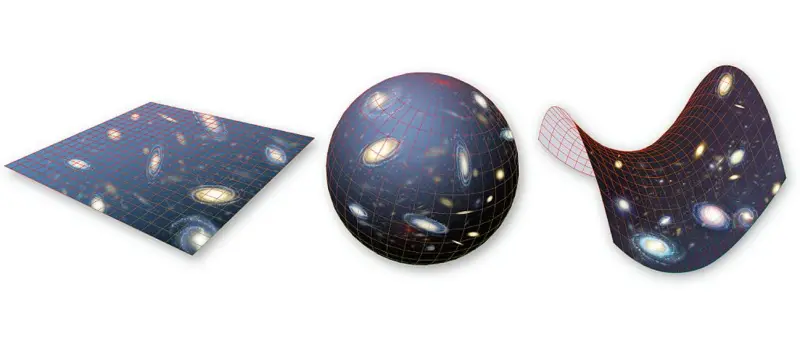
\includegraphics[scale=0.5]{curvaturuniverso.jpg}
\end{center}
\subsection*{Luz, curvatura y agujeros negros}
En geometría diferencial aplicada a relatividad, la trayectoria de un rayo de luz también se describe mediante una geodésica, pero de tipo \textit{nulo}: el vector tangente $\dot{\gamma}$ satisface $g(\dot{\gamma}, \dot{\gamma}) = 0$. Esto significa que incluso la luz sigue “el camino más recto posible” según la geometría del espaciotiempo. Por tanto, una gran masa (como una estrella o un agujero negro) puede desviar la luz, como lo demuestra el fenómeno del \textit{lente gravitacional}.\\
La idea de \textit{velocidad de escape} se puede reinterpretar desde este marco geométrico. Si un cuerpo es tan masivo y denso que la velocidad de escape desde su superficie iguala la velocidad de la luz, entonces ni siquiera la luz puede escapar: se forma un \textit{agujero negro}. El \textit{radio de Schwarzschild} se define como:
\begin{align*}
  r_s = \frac{2GM}{c^2}, 
\end{align*}
y corresponde a un horizonte de eventos: una superficie límite donde todas las geodésicas nulas convergen hacia el interior del agujero negro.
\subsection*{Analogías geométricas y visualización}
Para hacer accesible esta teoría, se suele emplear una analogía con una \textit{membrana elástica}. Imaginemos una lona de caucho donde colocamos una bola pesada que deforma su superficie. Si lanzamos otra bola cercana, esta no se moverá en línea recta, sino que seguirá una curva determinada por la deformación: está siguiendo una geodésica en un espacio curvado. Esta imagen, aunque bidimensional y clásica, ayuda a comprender cómo la materia y la geometría están profundamente entrelazadas.
%%%%%%%%%%%%%%%%%%%%%%%%%%%%%%%%%%%%%%%%%%%%%%%%%%
\section{Formación de agujeros negros desde la geometría diferencial}

\subsection{Variedades pseudo-riemannianas}

Una \textbf{variedad pseudo-riemanniana} \((M, g)\) es una variedad diferenciable donde el tensor métrico \(g\) es simétrico, no degenerado y no positivo definido. Esto significa que, a diferencia de la métrica riemanniana (positiva definida), la métrica pseudo-riemanniana permite medir intervalos que pueden ser positivos, negativos o nulos, dependiendo de la dirección del vector.

\subsection{Espaciotiempo como variedad lorentziana}

En relatividad general, el espaciotiempo es modelado como una \textbf{variedad lorentziana} de dimensión 4, con una métrica de firma \((-+++) \). Dada esta estructura, el cuadrado del intervalo entre dos eventos está dado por:

\begin{align*}
ds^2 = g_{\mu\nu} dx^\mu dx^\nu
\end{align*}

Donde:
\begin{itemize}
  \item \(ds^2 < 0\): trayectoria tipo tiempo.
  \item \(ds^2 = 0\): trayectoria tipo luz.
  \item \(ds^2 > 0\): trayectoria tipo espacio.
\end{itemize}

\subsection{Curvatura del espaciotiempo}

La curvatura se describe mediante el \textbf{tensor de Riemann}:

\begin{align*}
R^\rho_{\ \sigma\mu\nu} = \partial_\mu \Gamma^\rho_{\nu\sigma} - \partial_\nu \Gamma^\rho_{\mu\sigma} + \Gamma^\rho_{\mu\lambda} \Gamma^\lambda_{\nu\sigma} - \Gamma^\rho_{\nu\lambda} \Gamma^\lambda_{\mu\sigma}
\end{align*}

Este tensor mide cómo cambia un vector cuando se transporta paralelamente a lo largo de un lazo cerrado en la variedad.

Dos contracciones importantes del tensor de Riemann son:

\begin{itemize}
  \item \textbf{Tensor de Ricci}:
  \begin{align*}
  R_{\mu\nu} = R^\lambda_{\ \mu\lambda\nu}
  \end{align*}
  \item \textbf{Escalar de curvatura}:
  \begin{align*}
  R = g^{\mu\nu} R_{\mu\nu}
  \end{align*}
\end{itemize}

\subsection{Ecuaciones de Einstein}

Las ecuaciones de campo de Einstein relacionan la geometría del espaciotiempo con su contenido de materia y energía:

\begin{align*}
R_{\mu\nu} - \frac{1}{2} R g_{\mu\nu} = \frac{8\pi G}{c^4} T_{\mu\nu}
\end{align*}

\begin{itemize}
  \item El lado izquierdo representa la curvatura del espaciotiempo.
  \item El lado derecho describe el contenido de materia y energía mediante el tensor energía-momento \(T_{\mu\nu}\).
\end{itemize}

\subsection{Solución de Schwarzschild}

En el caso de simetría esférica en vacío (\(T_{\mu\nu} = 0\)), se obtiene la métrica de Schwarzschild:

\begin{align*}
ds^2 = -\left(1 - \frac{2GM}{c^2 r} \right)c^2 dt^2 + \left(1 - \frac{2GM}{c^2 r} \right)^{-1} dr^2 + r^2 d\Omega^2
\end{align*}

donde \(d\Omega^2 = d\theta^2 + \sin^2\theta d\phi^2\) representa el elemento de área de la esfera.

La cantidad:

\begin{align*}
r_s = \frac{2GM}{c^2}
\end{align*}

se llama \textbf{radio de Schwarzschild}. Si un cuerpo colapsa bajo este radio, se forma un \textbf{agujero negro}.

\subsection{Horizonte de eventos y singularidad}

\begin{itemize}
  \item El \textbf{horizonte de eventos} se encuentra en \(r = r_s\). A partir de allí, ninguna señal o partícula puede escapar al infinito.
  \item En \(r = 0\) hay una \textbf{singularidad} donde las cantidades geométricas como la curvatura se vuelven infinitas.
\end{itemize}

\subsection{Interpretación geométrica}

Desde la geometría diferencial, un \textbf{agujero negro} es una región del espaciotiempo cuya curvatura es tan intensa que altera la estructura causal. Las geodésicas temporales dentro del horizonte están todas dirigidas hacia la singularidad. Esto implica que, una vez cruzado el horizonte, el “futuro” inevitable de cualquier partícula es alcanzar el centro, lo cual no es una elección sino una consecuencia geométrica.

Así, los agujeros negros no son objetos “físicos” en el sentido clásico, sino regiones definidas por la \textbf{estructura geométrica} del espaciotiempo, determinada por las ecuaciones de Einstein.

\begin{center}
  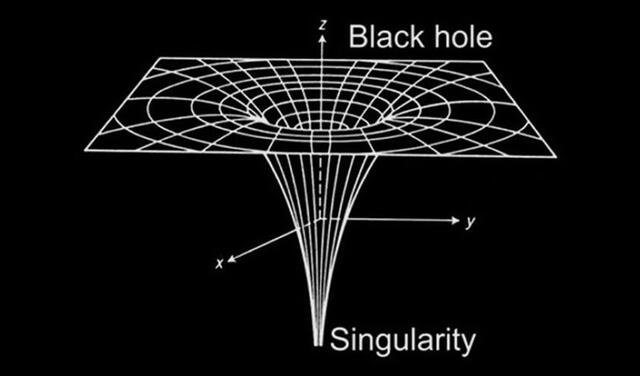
\includegraphics[scale=0.5]{negroagujero.jpeg}
\end{center}

%%%%%%%%%%%%%%%%%%%%%%%%%%%%%%%%%%%%%%%%%%%%%%%5
\section{Implicaciones}
\subsection*{La geometría del espacio determina la estructura y el destino del universo}
En geometría diferencial, la curvatura escalar—o más generalmente, la curvatura seccional—afecta directamente las propiedades locales y globales de una variedad. Según el artículo, dependiendo de si la curvatura del universo es positiva, nula o negativa, varían la suma de los ángulos de un triángulo, el comportamiento de las geodésicas y el volumen de las regiones espaciales.\\
Desde un punto de vista cosmológico, esta clasificación tiene consecuencias dinámicas:
\begin{itemize}
  \item Un \textbf{universo cerrado} ($K > 0$) podría colapsar en un “Big Crunch”.
  \item Un \textbf{universo plano} ($K = 0$) se expande para siempre, pero desacelerando.
  \item Un \textbf{universo abierto} ($K < 0$) se expande indefinidamente y de forma acelerada.
\end{itemize}
Así, la geometría del espacio tiene consecuencias físicas observables. Comprender la curvatura del universo es esencial para predecir su evolución a largo plazo.
\subsection*{Los agujeros negros surgen naturalmente del análisis geométrico}
El artículo explica que si la velocidad de escape de un cuerpo celeste es igual a la velocidad de la luz, entonces ni siquiera la luz puede escapar de su campo gravitatorio. Esto conduce al concepto de \textit{agujero negro}, una región del espaciotiempo donde la curvatura es tan extrema que todas las geodésicas nulas convergen hacia el interior.\\
Esta condición está definida por el radio de Schwarzschild:
\begin{align*}
r_s = \frac{2GM}{c^2}.
\end{align*}
Lejos de ser una anomalía física exótica, un agujero negro es una estructura geométrica que surge naturalmente de las ecuaciones de Einstein. Representa una región donde la curvatura del espaciotiempo obliga a todas las trayectorias causales a dirigirse hacia el interior.\\
Por lo tanto, los agujeros negros no son singularidades en el sentido de fallas de la física, sino consecuencias naturales de la geometría diferencial del espaciotiempo bajo campos gravitacionales intensos.
%%%%%%%%%%%%%%%%%%%%%%%%%%%%%%%%%%%%%%%%%%%%%%%
\section{Conclusiones}
El estudio del universo desde la perspectiva de la geometría diferencial permite una comprensión profunda y unificada de fenómenos físicos fundamentales.\\
A través del análisis de geodésicas, curvatura y estructuras métricas, se logra reinterpretar la gravedad no como una fuerza, sino como el resultado de la curvatura del espaciotiempo inducida por la materia y la energía.\\
Los modelos cosmológicos basados en curvatura constante (cerrado, plano y abierto) muestran cómo la geometría global afecta el destino dinámico del universo.\\
Además, conceptos como los agujeros negros, que antes eran considerados exóticos o paradójicos, surgen de manera natural como soluciones geométricas dentro del marco de la relatividad general.\\
Este enfoque no solo ofrece elegancia y coherencia teórica, sino que también permite predicciones precisas que han sido confirmadas experimentalmente, como la deflexión de la luz por la gravedad o la detección de ondas gravitacionales.\\
La geometría diferencial, por tanto, no es solo una herramienta matemática, sino un lenguaje esencial para describir la realidad física del cosmos.
%%%%%%%%%%%%%%%%%%%%%%%%%%%%%%%%%%%%%%%%%%%%%%%
\newpage
\nocite{*}
\printbibliography

\end{document}
